% Chapter Template

\chapter{Methodology} % Main chapter title

\label{Chapter4} % Change X to a consecutive number; for referencing this chapter elsewhere, use \ref{ChapterX}

\lhead{Chapter 5. \emph{Methodology}} % Change X to a consecutive number; this is for the header on each page - perhaps a shortened title

%----------------------------------------------------------------------------------------
%	SECTION 1
%----------------------------------------------------------------------------------------

\section{Many-body Methods}

As previously discussed in Chapter \ref{Chapter1}, the aim of many-body quantum mechanics 
is to find either the exact, or a reliable
approximation to the many-body systems wave function $\Psi$. In methods like coupled cluster theory, this wave
function resides in Fock space, a space spanned by all possible Slater
determinants constructed by the single-particle states from the
corresponding one-body problem. This wave function may be written (for
$N$ particles)
\begin{equation}
\vert \Psi \rangle = c_0 \vert \Phi_0 \rangle + \sum_{ai} c_{ai }\vert \Phi_i^a \rangle +  \sum_{abij} c_{abij} \vert \Phi_{ij}^{ab} \rangle + ... + \sum_{ab...N_a ij...N_i} c_{ab...N_a ij...N_i} \vert \Phi_{ij...N_i}^{ab...N_a} \rangle.
\label{eqn:fullCI}
\end{equation}

To determine the full wave function we therefore need a complete
single-particle basis as well as the means to project it onto Fock
space, determining its coefficients. In general, we may consider the
process of generating the full wave function from the reference state
to be an operator $\hat{\Omega}$ acting on the reference state
\begin{equation}
\vert \Psi \rangle = \hat{\Omega} \vert \Phi_0 \rangle .
\label{eqn:reference_operator}
\end{equation}

The explicit form of $\hat{\Omega}$ is to be determined by the various many-body methods. 

\section{The Hartree-Fock Method}

A complete basis often means an infinite number of single-particle
states, which in turn means an infinite number of Slater
determinants. Such a system is not possible to implement
computationally, so we may instead seek ways of truncating our
basis. As previously discussed in chapters 1 and 2, the precision of
our solution will now depend on how much of the exact wave function is
present in the retained basis. To this end, we will seek a
single-particle basis that ensures that most, or as much as possible,  of the systems wave
function is present in one single Slater determinant.

The \emph{Hartree-Fock method} is a way of optimizing the
single-particle states so that a single Slater determinant gives a
good representation of the system. The resulting Slater determinant
may serve as a starting point for several so called \emph{post Hartree-Fock methods}, 
such as MBPT (many body perturbation theory),
CI (Configuration Interaction) or CC (Coupled Cluster)
method \cite{ShavittBartlett2009}.

The first development of the method is attributed to Douglas Rayner
Hartree who in 1927 introduced a procedure he called 
\emph{the self  consistent field method} \cite{Thijssen} but which was later named
the \emph{Hartree-Fock-Rothaan} method. Some of the original differences between various Hartree-Fock approaches 
are nowadays seldomly mentioned or have simply been forgotten \cite{ShavittBartlett2009},
and the more generic name Hartree-Fock normally refers to the method that will be discussed in
the following sections.

\subsection{The variational principle}

The Hartree-Fock method is based on the variational principle, which
states that when we evaluate the inner product of the Hamiltonian on
\emph{any} normalized wave function, the resulting energy will be an
upper bound to the ground state energy \cite{Griffiths2005},
that is
\begin{equation}
E_0 \leq \langle \Psi_{trial} \vert \hat{H} \vert \Psi_{trial} \rangle.
\label{eqn:variational}
\end{equation}

Such wave functions are commonly called \emph{trial} wave functions. 

The variational principle provides us with an approximate scheme, and
by parameterizing the trial wave function we may improve upon this
solution.

\subsection{Expanding the single-particle states}

The parametrization of the Slater determinant may be performed by letting
each single-particle state be represented by a linear combination of
the eigenstates to the corresponding one-body problem. If we refer to
the linear combinations by $\psi$ with Latin indices and the basis
states as $\phi$ with Greek indices, we may write this as
\begin{equation}
\vert \psi_i \rangle = \sum_\alpha^A c_{\alpha,i} \vert \phi_{\alpha,i} \rangle .
\label{eqn:expanding_sp_states}
\end{equation}

Note that we truncate the basis at the A'th function to make
computations possible. More functions generally means a better
representation. In principle, our basis sets span an infinity of states, but due to obvious computational limits we have to truncate the above sum.

In accordance with the variational principle, we now want to determine
the coefficients $c_{\alpha, i}$ in such a way that we minimize the
energy. We should therefore insert the expanded single-particle states
into the energy equation (\ref{eqn:many_body_energy}) that we derived
in chapter 1. We will assume that the system's Hamiltonian has the form

\begin{equation}
\hat{H} = \hat{H}_0 + \hat{H}_I = \sum_{i=1}^N \hat{h}_0(\mathbf{x}_i) + \sum_{i<j=1}^N \hat{v}(\mathbf{x}_i,\mathbf{x}_j),
\end{equation}

where $N$ is the number of particles in our system,  $\hat{h}_0(\mathbf{x}_i)$ is the one body operator acting on particle $i$, and $\hat{H}_I$ is the interaction. For simplicity, we will avoid defining these in more detail, and we will use the following shorthand notation for the two-body integrals

\begin{equation}
\langle \alpha \beta \vert V \vert \alpha \beta \rangle \equiv \int \psi_\alpha^*(\mathbf{r}_i) \psi_\beta^*(\mathbf{r}_j) V(r_{ij})  \psi_\alpha(\mathbf{r}_i) \psi_\beta(\mathbf{r}_j) d\mathbf{r}_i\mathbf{r}_j,
\end{equation}

\begin{equation}
\langle \alpha \beta \vert V \beta \alpha \rangle \equiv \int \psi_\alpha^*(\mathbf{r}_i) \psi_\beta^*(\mathbf{r}_j) V(r_{ij})  \psi_\alpha(\mathbf{r}_j) \psi_\beta(\mathbf{r}_i) d\mathbf{r}_i\mathbf{r}_j,
\end{equation}

Where the quantity $r_{ij} = \vert \mathbf{r}_i - \mathbf{r}_j \vert$ indicates that the interaction depends upon the distance between the particles. We may even express this as an antisymmetric matrix element:

\begin{equation}
\langle \alpha \beta \vert V \vert \alpha \beta \rangle_{AS}  \equiv \langle \alpha \beta \vert V \vert \alpha \beta \rangle - \langle \alpha \beta \vert V \vert \alpha \beta \rangle.
\end{equation}

By inserting the expanded states in Eqn. \ref{eqn:many_body_energy}, we will find the eigenvalue of the Hamiltonian expressed as a function of the set of coefficients $\{c\}$
\begin{multline}
 \epsilon (\{c\}) = \sum _{\alpha, \beta}^A c_{\alpha,i}^{*}c_{\beta,i} \sum _{i}^N \langle \phi _\alpha | \hat{h}_0 | \phi _\beta \rangle + \\ 
 \sum _{\alpha,\beta, \gamma, \delta} ^A c_{\alpha,i}^{*}c_{\beta,j}^{*}c_{\gamma,i}c_{\delta,j}
 \frac{1}{2} \sum _{i=1,j=1}^N \langle \phi _{\alpha}\phi _{\beta}| \hat{v} |\phi _{\gamma}\phi _{\delta} \rangle_{AS}.
\label{eqn:greek_HF}
\end{multline}

The way in which we now have set up the system, we may consider the
coefficients to be a matrix with $A$ rows (Greek letters) and $N$
columns, where $N$ is the number of particles. In the special case
where diagonal elements are one and all others zero, we find the same
system as we have discussed up to this point.

\subsection{Ensuring orthonormality}

The trial wave function is now parameterized by the introduction of
coefficients. When varying or optimizing these coefficients to
minimize the energy, we must be careful to constrain the
orthonormality of the states (remember, failing to do so will cause a
violation of the Pauli principle). Mathematically this constraint may
be written
\begin{equation}
\langle \psi_i \vert \psi_j \rangle = \sum_{\alpha}^A c_{\alpha, i}^*c_{\alpha, j} = \delta_{ij}.
\label{eqn:orthonormality}
\end{equation}

To this end, we may use \emph{Lagrange's method of undetermined  multipliers} \cite[p.116]{Szabo} 
(or simply \emph{Lagrange  multipliers}), and set up a functional to be minimized with the
constraint described above, namely
\begin{equation}
 F\big( \epsilon \big( \{c\} \big), \lambda \big) =  \epsilon \big( \{c\} \big) - \sum _i^N \lambda _i \sum _{\alpha}^A c_{\alpha,i}^{*} c_{\alpha,i}.
 \label{lagrange_minim}
\end{equation}

To find a minimum for this functional we must solve
\begin{equation}
\frac{\partial}{\partial c_{\alpha,i}^{*}} F\big(  \epsilon \big( \{c\} \big), \lambda \big) = 0.
\label{eqn:partialset}
\end{equation}

For a step by step solution, the reader is referred to Thijssen's
\emph{Computational Physics} \cite{Thijssen} or Szabo's \emph{"Modern Quantum Chemistry"} \cite{Szabo}. 
In the following we will just
state the solution consistent with how it is given in these sources.

\subsection{The Hartree-Fock Equations}

By solving Eq.~(\ref{eqn:partialset}), we obtain a set of coupled one particle eigenvalue problems given by

\begin{multline}
\lambda _k c_{\alpha,k} =  
\sum _{\gamma}^A\sum _{i}^N c_{\gamma,k}\langle \alpha |\hat{h}_0| \gamma \rangle + 
\sum _{\beta,\gamma,\delta}^A \sum _i^N c_{\beta,i}^{*}c_{\gamma,i}c_{\delta,k}\langle \alpha \beta | V |\gamma \delta \rangle_{AS}.
 \label{eqn:HF1}
\end{multline}

These are known as the Hartree-Fock equations, and by identifying $\lambda$ as energy associated with single-particle state k \cite{hh4480} we may write them as
\begin{equation}
\epsilon_k^{HF} c_{\alpha,k} =  
\sum_{\gamma} \Big{(}  {\langle \alpha |\hat{h}_0 | \gamma \rangle + 
\sum_j^N \sum_{\beta \delta}{c_{j \beta} c_{j \delta}  \langle \alpha \beta | V | \gamma \delta \rangle_{AS} } } \Big{)} c_{ \gamma, k},
 \label{eqn:HF2}
\end{equation}

or simply 

\begin{equation}
\sum_\gamma f_{\alpha \gamma}^{HF} c_{\gamma,k} = \epsilon_k^{HF} c_{k,\alpha},
\label{eqn:hartreefock}
\end{equation}

where we defined

\begin{equation}
 f_{\alpha \gamma}^{HF}  \equiv   \langle \alpha |\hat{h}_0 | \gamma \rangle + 
\sum_j^N \sum_{\beta \delta}{c_{j \beta} c_{j \delta}  \langle \alpha \beta | V | \gamma \delta \rangle_{AS} } 
 \label{eqn:HF2}
\end{equation}

The matrix $ \hat{f}^{HF} $ is commonly known as the \emph{Fock}
matrix, and has dependence upon all the spin
orbitals. \cite{ShavittBartlett2009}. As a consequence, a first guess
for the coefficients is likely to be inconsistent when evaluating the
left hand side and right hand side of Eq.~(\ref{eqn:hartreefock}), so they
are normally solved in an iterative manner. This is why the method was
initially named the self-consistent field method; the field produced
by the particles should be consistent with the field "felt" by each
particle.

A set of single particle states that fulfills Eq.~(\ref{eqn:hartreefock})
are called the \emph{canonical Hartree-Fock wave function}, while the
constituent states are called \emph{the canonical spin orbitals}.

\subsection{Koopman's theorem}

The Hartree Fock energy for any single-particle state $p$ may be compactly written
\begin{equation}
\epsilon^{HF}_p = \langle p \vert \hat{h}_0 \vert p \rangle + \frac{1}{2} \sum_{j} \langle pj \vert  \vert pj \rangle .
\label{eqn:hf_koopman}
\end{equation}

This is the energy associated with each orbital expanded as a linear combination of single-particle states. Each fermion in the system will then have an associated Hartree-Fock energy.

Koopman's theorem states that for closed-shell Hartree-Fock
calculations, the ionization energy of the system is equal to the
negative of the outermost hole state in the reference state. \cite{Thijssen}
The ionization energy may then be computed by performing a Hartree-Fock procedure, 
whereby we calculate only the outermost occupied
orbital in equation Eq.~(\ref{eqn:hf_koopman}).

\subsection{Restricted and unrestricted Hartree-Fock}

There are multiple ways of implementing the Hartree-Fock
equations. For closed shell systems, such as $He$, $H_2$ and $Be$, the
electrons (we consider only electronic degrees of freedom in this thesis), may be assumed to be paired with
opposite spin electrons. In the restricted Hartree-Fock method (RHF),
we consider only systems where all fermions (electrons in our case) are paired with opposite
spin particles. This lets us scale down the computation, but it will
naturally give poor results for systems where no such pairing occurs,
for example in the case where two $H$ atoms are interacting over
large distances.

For systems with singly occupied states (unpaired fermions, typically
odd numbered systems) the restriction of spin-pairing is no longer valid.

To take this into account, we set up two Fock matrices; one for each
spin orientation. The resulting system is
\begin{equation}
\hat{F}_\alpha(C_\alpha, C_\beta) C_\alpha = \hat{S} C_\alpha \epsilon_\alpha,
\end{equation}
and
\begin{equation}
\hat{F}_\beta(C_\alpha, C_\beta) C_\beta = \hat{S} C_\beta \epsilon_\beta.
\end{equation}

The subindices $\alpha$ and $\beta$ makes the distinction between the two possible spin-orientations in our system, for example $\alpha$ for spin up and $\beta$ for spin down. For each orientations we have a separate coefficient matrix $C$.

The ground state energy will be a function of the eigenvectors of
these two matrices. The dependency of opposite spin coefficients in
the Fock matrices is due to the direct- or coulomb term from the two
particle integrals \cite[p.241]{Szabo}. This latter approach is called
the \emph{unrestricted Hartree-Fock} (UHF) method.



\section{Post Hartree-Fock Methods}

While the Hartree-Fock reference state may account for important
correlations such as the Pauli exclusion principle and interactions
with the mean field, it will lack the more complicated correlations. For this reason, certain correlations may never
be fully accounted for with the Hartree-Fock method alone. Figure
\ref{fig:correlation} illustrates what is often defined as the
correlation energy; the energy attributed to correlations beyond the
mean field.
\begin{figure}[p]
    \centering
    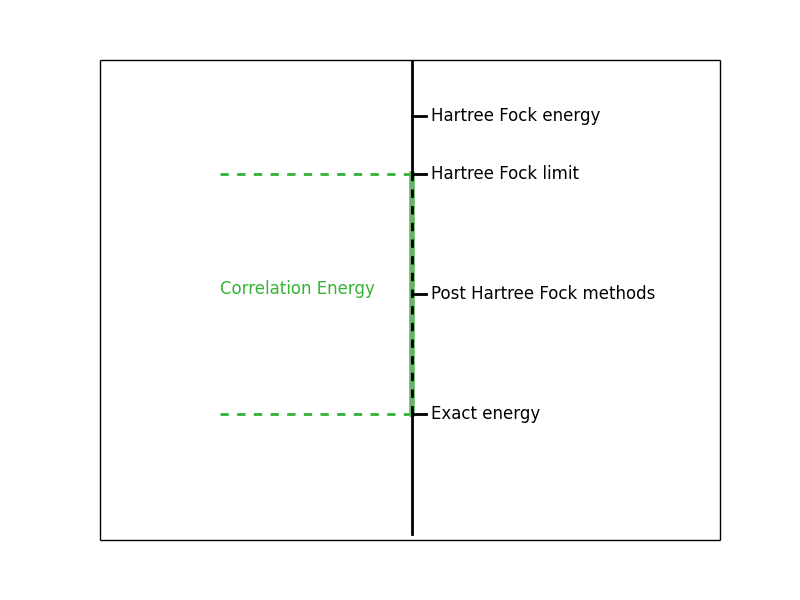
\includegraphics[width=0.8\textwidth]{correlation}
    \caption{Correlations beyond the Hartree-Fock energy. At the so
      called Hartree-Fock limit, we have achieved the best possible
      description of our system using the mean field approach. The
      energy unaccounted for by the reference state is commonly
      referred to as the \emph{correlation energy}. The so called
      \emph{post Hartree-Fock} methods, such as the Coupled Cluster
      method, will help us include even more correlations and bring us
      closer to the exact energy.}
    \label{fig:correlation}
\end{figure}

A Hartree-Fock calculation may also provide us with energy minimized orbitals above the Fermi level that may be used to construct excited Slater determinants in so-called \emph{post Hatree Fock} methods. 

By including excited Slater determinants, these methods may
account for the correlations beyond the mean field. One such approach is the Coupled Cluster (CC) method, which
is a central subject in this thesis. Alongside CC, we have several
other methods such as Configuration Interaction (CI) or Many Body
Perturbation Theory (MBPT).

Important insight into various physical systems may be gained by
comparing results amongst these methods, as they all have their
strengths and weaknesses. Prior to the treatment of the CC method in
chapter 5, we shall therefore just briefly discuss some of these
alternative post Hartree-Fock methods, allowing us to make a meaningful comparison of
results in the final chapter of this thesis.

\subsection{Configuration Interaction theory}

The Configuration Interaction (CI) method, sometimes referred to as
the \emph{method of superposition of configurations} \cite{Harris} is
based on the expansion of the system's wave function into a linear
combination consisting of the reference Slater determinant and a
(possibly infinite) set of excited versions of this Slater
determinant, as briefly noted in the introduction to this chapter,
\begin{equation}
\vert \Psi \rangle = c_0 \vert \Phi_0 \rangle + \sum_{ai} c^{a}_i\ vert \Phi_i^a \rangle +  \sum_{abij} c^{ab}_{ij} \vert \Phi_{ij}^{ab} \rangle + ... + \sum_{ab...N_a ij...N_i} c^{ab...N_a}_{ij...N_i} \vert \Phi_{ij...N_i}^{ab...N_a} \rangle.
\label{eqn:fullCI}
\end{equation}

The CI method is considered to be the mathematically simplest
technique for inclusion of correlations beyond the mean
field \cite{Harris}. The operator that brings us from the reference
Slater determinant to the true system wave function may be written
\begin{equation}
\vert \Psi \rangle = \Omega \vert  \Phi_0 \rangle = (c_0 + \hat{C}) \vert  \Phi_0 \rangle,
\end{equation}
where
\begin{equation}
\hat{C} = \sum_{ai} c^{a}_i \Cr{a} \An{i}+  \sum_{abij} c^{ab}_{ij} \Cr{a} \Cr{b} \An{j} \An{i} + ... + \sum_{ab...N_a ij...N_i} c^{ab...N_a}_{ij...N_i} \Cr{a} \Cr{b} ... \Cr{N_a} \An{N_i} ... \An{j} \An{i}.
\end{equation}

The coefficients $c$ are then obtained by diagonalization, which corresponds to  minimizing 
\begin{equation}
E = \langle \Psi \vert \hat{H} \vert \Psi \rangle.
\label{eqn:fullCIvar}
\end{equation}

We shall not go into more details concerning this. The reader is
referred to for example \cite[p.177]{Harris} for a more complete
treatment.

We will however make some general observations concerning the CI method. 

\subsection{Full Configuration Interaction theory}

Equation (\ref{eqn:fullCIvar}) is solvable, but at great
computational cost. The number of excited Slater determinants, and
thereby the number of coefficients, scales \emph{factorially} with the
number of particle states and hole states.

The practical consequence is that the inclusion of all Slater
determinants is only possible for smaller systems unless some
truncation in the basis set is introduced. From a physical
point of view, we may have systems where no single excitation is
allowed, and for this reason the singly excited coefficients may be
excluded with no loss of precision.

The various truncations are commonly referred to as CIS for inclusion
of single excitations, CISD for single and double excitations and so
on.

\subsection{Configuration Interaction Quantum Monte Carlo}

We will later in this thesis compare results with results from a
so-called FCIQMC (Full Configuration Interaction Quantum Monte Carlo)
calculation. This approach determines the FCI coefficients by
stochastic processes \cite{Booth2013,Leikanger2013}. Such
results are valuable for our purpose, since they basically provide us
with the exact ground state energy for smaller systems, which will
allow us to evaluate to which degree the method accounts for
correlations in the system.

\subsection{Many Body Perturbation Theory}

As opposed to the Hartree-Fock, Configuration Interaction and
Coupled Cluster methods, \emph{Many Body Perturbation Theory} (MBPT)
offers a non-iterative approach to approximating the systems wave
function. The following derivation is based on the one in Refs.
\cite{ShavittBartlett2009} and \cite{hh4480}.

The basic idea is to arrange the Hamiltonian into two parts
\begin{equation}
\hat{H} = \hat{H}_0 + \hat{V}.
\end{equation}

This is very similar to what we have done so far, as we seek an
operator $\hat{H}_0$ which is exactly solvable (which yields the
single-particle basis) and an operator $\hat{V}$ that will be treated as a
perturbation. The solution to the unperturbed problem is given
\begin{equation}
\hat{H}_0 \vert \Phi_0 \rangle = W_0 \vert \Phi_0 \rangle.
\end{equation}

As for Configuration Interaction theory, we have the exact ground state wave
function for our system represented by a linear combination of Slater
determinants, where we assume the first term (reference state) to be
the dominating term
\begin{equation}
\vert \Psi_0 \rangle = \vert \Phi_0 \rangle + \sum_m^\infty c_m \vert \Phi_m \rangle.
\end{equation}
 
We then assume intermediate normalization $\langle \Phi_0 \vert
\Psi_0 \rangle = 1$ and project our Schödinger equation onto $\langle
\Phi_0 \vert$ :
\begin{equation}
\langle \Phi_0 \vert \hat{H} \vert \Psi_0 \rangle = \langle \Phi_0 \vert \hat{H}_0 + \hat{V} \vert \Psi_0 \rangle = E.
\end{equation}

The true ground state energy is still unknown, but we
may subtract the \emph{unperturbed} energy to find an expression for
the correlation energy
\begin{equation}
\langle \Phi_0 \vert \hat{V} \vert \Psi_0 \rangle = E - W_0 = \Delta E.
\end{equation}

We may add and subtract a term $\omega \vert \Psi_0 \rangle$ to the expression above and regroup it to find
\begin{equation}
\vert \Psi_0  \rangle = \frac{1}{(\omega - \hat{H}_0)} (\hat{V} + \omega - E) \vert \Psi_0 \rangle .
\label{eqn:pt_1}
\end{equation}

By interpreting the term $\omega$ in different ways, we will arrive at the various many-body perturbation schemes.

The system's true wave function is still unknown, but it is fully
possible to expand it in a known basis $\{\phi_n \}$, so that
\begin{equation}
\vert \Psi \rangle = (\hat{P} + \hat{Q})\vert \phi_0 \rangle,
\end{equation}
where we have the projection operator $\hat{P} = \vert \phi_0 \rangle \langle \phi_0 \vert$, $\hat{P} = \hat{P}^\dagger = \hat{P}\hat{P}$ and $\hat{Q} = \sum_{m} \vert \phi_m \rangle \langle \phi_m \vert$ \cite{ShavittBartlett2009}. 
We insert this into Eq. (\ref{eqn:pt_1}) to find
\begin{equation}
\vert \Psi_0  \rangle = \phi_0 \rangle + \sum_i^\infty \Big{(} \frac{1}{(\omega - \hat{H}_0)} (\hat{V} + \omega - E) \Big{)}^i \vert \phi_0 \rangle ,
\label{eqn:pt_2}
\end{equation}
and the correlation energy takes the form
\begin{equation}
\Delta e = \sum_i^\infty  \hat{V} \Big{(} \frac{1}{(\omega - \hat{H}_0)} (\hat{V} + \omega - E) \Big{)}^i \vert \phi_0 \rangle .
\label{eqn:pt_2}
\end{equation}

By letting $\omega = E$, we obtain the so called Brillouin-Wigner
Perturbation Theory, or we may let $\omega = W_0$ to obtain
Rayleigh-Schrödinger Perturbation Theory (RSPT). In the
Brillouin-Wigner case, a possible solution would involve iterations
and self consistence as in the Hartree-Fock-, Configuration Interaction- and Coupled Cluster cases, while in the RSPT
case we end up with terms that correspond to different orders of the
correlation energy. For RSPT, we obtain
\begin{equation}
\Delta e = \Delta E^{(1)}+\Delta E^{(2)}+\Delta E^{(3)}+... ,
\end{equation}
where
\begin{equation}
\Delta E^{1} = \langle \phi_0 \vert \hat{V} \vert \phi_0 \rangle,
\end{equation}
\begin{equation}
\Delta E^{2} = \langle \phi_0 \vert \hat{V}  \frac{\hat{Q}}{(W_0 - \hat{H}_0)}  (\hat{V} - \Delta E) \vert \phi_0 \rangle,
\end{equation}
\begin{equation}
\Delta E^{3} = \langle \phi_0 \vert \hat{V} \frac{\hat{Q}}{(W_0 - \hat{H}_0)}  (\hat{V} - \Delta E) \frac{\hat{Q}}{(W_0 - \hat{H}_0)}  (\hat{V} - \Delta E)  \vert \phi_0 \rangle,
\end{equation}
represent the correlation energy to first, second and third order, respectively. Higher orders are obtained along similar lines. Every order in RSPT introduces different types of correlations. With a two-body force only, to second order we can obtain contributions from at most two-particle-two-hole excitations. At for example fourth order, we can also obtain contributions
which represent four-particle-four-hole  excitations.  
Whereas methods like Configuration Interaction or Coupled Cluster include such correlations 
to infinite order in the interaction, RSPT contains such correlations only up to the given order in the expansion.



\subsection{The linked diagram theorem}

We will not go into any further detail on the many-body perturbation
methods, but we should note an important theorem introduced by
Goldstone \cite{Goldstone1957}, see also Ref.~\cite[p.152]{ShavittBartlett2009}.

Computations of the different orders in Rayleigh-Schrödinger
Perturbation Theory may be performed diagrammatically. Based on a set
of rules (see for example \cite{ShavittBartlett2009}), we may generate
diagrams corresponding to the possible contractions operators
present in each order of the perturbation. Actually, the diagrammatic
rules will produce a lot more diagrams then what is actually needed in
order to calculate the correlation energy.

The \emph{linked diagram theorem} is a simple way of getting rid of a lot of these excess diagrams.

A diagram may be called \emph{linked} if all parts of the diagram is
linked with each other by contractions. Unlinked diagrams will be
easily identified as it is possible to split them into smaller parts
by drawing lines through them without crossing any lines in the
diagram.

The linked diagram theorem states that these diagrams do not contribute to the correlation energy. 

In Eq. (\ref{eqn:pt_2}) for Rayleigh-Schrödinger Perturbation Theory, we will therefore only have to consider terms where contractions occur for diagrams where every vertex is linked to another vertex by at least one particle or hole line.

\section{Other many-body methods}

The methods we have discussed so far are relevant to this thesis, but the full range of methods for dealing with many body problems extends even further. Some notable methods apart from the ones discussed so far is the wide range of \emph{Quantum Monte Carlo} (QMC) methods, that build upon the same formalism as us, but use instead stochastic methods to approximate the systems wavefunction (see for example \cite[Chapter 12]{Thijssen}). Other methods such as \emph{Density Functional Theory} (DFT) may even depart from the Hartree-Fock formalism to offer more suitable equations for solids, while at the same time represent alternatives to Hartree-Fock calculations for atoms and molecules \cite[Chapter 5]{Thijssen}.